\section{Implementation details}
\label{app:replication}

\subsection{Data preparation and splits}

For social allocation \citep{wang2026decomposing}, we corrected displaced column labels in the released spreadsheet: allocation responses were stored under \texttt{Warmth}. We checked the correction against the questionnaires in all eight country-by-wave-by-task samples and divided the recorded values by five to recover the 0--20 token scale. All reported analyses use the corrected responses.

For categorization \citep{cao2024differences}, we retained the authors' Experiment 2 sample (295 US and 178 Chinese participants), reconstructed choices from raw responses and the original stimulus key, and excluded 15 fillers and two attention checks. US participants answered in English and Chinese participants in Mandarin; models received English prompts. For risky choice \citep{anllo2024preferences}, we used phase 3, conditions 5--12 (50 US and 49 Chinese participants), without additional performance-based exclusions. All four repetitions and both display orders of a lottery pair were treated as one item.

For each seed (0, 1, 2), we sampled equal country pools without replacement and assigned 70\% to training, 15\% to validation, and the remainder to testing, rounding the first two counts down (Table~\ref{tab:replication-splits}). The giving variant was balanced and split within each wave. Selection did not use responses, and each participant's responses stayed together. Pooled adapters used half as many participants from each country's training pool, keeping the total training sample fixed; giving-variant pooled samples were not further stratified by wave. The validation set was unused: all results use the final checkpoint after 25 updates.

\begin{table}[htbp]
\centering\small
\begin{tabular}{lrrrr}
\toprule
Sample & Pool & Training & Validation & Test \\
\midrule
Social allocation: giving variant, wave 1 & 501 & 350 & 75 & 76 \\
Social allocation: giving variant, wave 2 & 800 & 560 & 120 & 120 \\
Categorization & 178 & 124 & 26 & 28 \\
Risky choice & 49 & 34 & 7 & 8 \\
\bottomrule
\end{tabular}
\caption{Participants per country and seed after balancing. Giving-variant totals are summed across waves. Participants are shared across item folds within a seed.}
\label{tab:replication-splits}
\end{table}

Item folds were fixed across countries and seeds: five folds of five social targets, five folds of three categorization items, and four folds containing one tradeoff and one dominance lottery pair. Translations, answer orders, and repetitions stayed in the same fold. Adapters fine-tuned on the giving variant predicted the excluded targets in both social allocation variants. Each item contributed once per seed, using the model fitted without that item; item and seed means received equal weight.

The taking variant was used only for evaluation. We retained all 1,329 Chinese participants and sampled 1,329 US participants without replacement, matching 529 per country in wave 1 and 800 in wave 2. The same sample was used for all model and human comparisons. Source files, preparation scripts, split and fold manifests, and runtime records are documented in the accompanying code's \path{REPRODUCING.txt}.

\subsection{Training}

We loaded the backbone and tokenizer from \href{https://huggingface.co/unsloth/Meta-Llama-3.1-70B-bnb-4bit}{\texttt{unsloth/Meta-Llama-3.1-70B-bnb-4bit}} and the original adapter from \href{https://huggingface.co/marcelbinz/Llama-3.1-Centaur-70B-adapter}{\texttt{marcelbinz/Llama-3.1-Centaur-70B-adapter}}. Base Llama evaluation disabled the Centaur adapter. The backbone and Centaur adapter stayed frozen during fine-tuning. The added population adapter initially contributed zero; its predictions matched frozen Centaur within $10^{-6}$ before training.

The rank-stabilized LoRA adapter used rank 8, $\alpha=8$, scaling $\alpha/\sqrt{r}$, no dropout, and no trainable biases. It targeted \texttt{q\_proj}, \texttt{k\_proj}, \texttt{v\_proj}, \texttt{o\_proj}, \texttt{gate\_proj}, \texttt{up\_proj}, and \texttt{down\_proj} in every transformer block. The backbone used 4-bit NF4 with double quantization and BF16 computation.

Each update minimized cross-entropy against empirical response frequencies across all training items: 20 giving-variant prompts, 24 categorization prompts, or 12 risky-choice prompts. Binary items appeared in both answer orders with equal total weight per item. Only the answer token contributed to loss, using full-vocabulary probabilities. AdamW used learning rate $5\times10^{-5}$, weight decay 0.01, $(\beta_1,\beta_2)=(0.9,0.999)$, and $\epsilon=10^{-8}$, without gradient clipping. Training ran for 25 updates, with three linear warmup updates followed by linear decay. The 768-token limit allowed left truncation for allocation, preserving the beginning-of-sequence token; longer binary inputs were rejected.

\subsection{Prompts and scoring}

Each item was presented independently as plain text. Allocation prompts used the English questionnaire instructions, one social target, the 21 valid answers, and the ending \texttt{You enter <<}. Full allocation templates are in \path{scripts/evaluate_dictator_giving_base.py} and \path{scripts/evaluate_dictator_taking_transfer.py}. The binary templates were:

\begin{quote}\small\ttfamily
Choose the option that is most closely related to the bolded item.\par
**\{cue\}**\\
A: \{option A\}\\
B: \{option B\}\par
You choose <<
\end{quote}

\begin{quote}\small\ttfamily
You are choosing between two lotteries. Each lottery pays the stated number of points with the stated probability and otherwise pays 0 points.\\
A: \{description A\}.\\
B: \{description B\}.\\
Which lottery do you choose? Respond with A or B.\\
You choose <<
\end{quote}

Lottery descriptions specified both outcomes, for example \texttt{10 points with a 25\% chance; 0 points with a 75\% chance}. Only the next answer token was scored: 0--20 or A/B. Probabilities were normalized over valid answers. For binary items, probabilities were mapped to the response meaning and averaged across answer orders before computing NLL. Training used full-vocabulary probabilities; evaluation used probabilities conditional on valid answers.

\subsection{Response adjustment}

For each population, seed, and fold, we fitted offsets shared across items to the same training responses as the adapter:
\[
q_{\delta}(y\mid x)=\frac{p_0(y\mid x)e^{\delta_y}}{\sum_k p_0(k\mid x)e^{\delta_k}},
\]
where $p_0$ is frozen Centaur's probability conditional on valid answers. We minimized mean training NLL plus $\lambda\sum_y\delta_y^2/2$, with $\lambda=0.001$ and offsets summing to zero. Allocation used 21 offsets; offsets fitted on the giving variant transferred unchanged to the taking variant. Binary choices used offsets $(d/2,-d/2)$, with positive $d$ favoring the taxonomic match or 10-point option. Training items and answer orders received equal weight.

The exploratory response adjustment with an answer-position parameter added a position offset $b$: the taxonomic match's or 10-point option's logit was $z_{\mathrm{AB}}+d+b$ when listed first and $z_{\mathrm{BA}}+d-b$ when listed second, where $z$ denotes frozen Centaur's logit for that response. The penalty was $\lambda(d^2+b^2)/4$. Both controls used training data only, with no test-based parameter selection. Adjustments were applied before averaging probabilities across orders. Positive values of adjustment NLL minus fine-tuned-model NLL favor fine-tuning.

\subsection{Uncertainty}

We used 4,000 percentile bootstrap resamples of participants within country, and within wave for allocation. Each participant's responses stayed together, with the same resampling weight across models, items, and overlapping seed splits. Each seed's score was normalized over its test participants before averaging seeds equally. Frozen-model intervals resampled the evaluated participants; categorization and risky-choice H1 analyses used all retained participants.

Allocation adapter comparisons also resampled the three observed seeds. Binary-task intervals held fits and seeds fixed; variation across seeds was reported separately. Human allocation differences retained the observed wave weights. All intervals are exploratory, pointwise 95\% intervals without multiplicity correction. They condition on the evaluated items and existing fits and do not account for new training samples or items.

\section{Additional results}
\label{app:additional-results}

\paragraph{Predictive scores.}
Table~\ref{tab:extension-scores} reports binary-task scores. Chinese fine-tuning improved prediction of Chinese responses in the giving variant of social allocation over US fine-tuning by 0.144 nats [0.105, 0.179]. Gains over frozen Centaur from matched fine-tuning were 0.053 [0.016, 0.087] and 0.021 [-0.019, 0.060] nats for US and Chinese categorization, and 0.031 [-0.017, 0.073] and 0.167 [0.069, 0.258] for risky-choice tradeoff pairs. Both matched-versus-pooled intervals for risky-choice tradeoff pairs included zero.

\begin{figure}[htbp]
\centering
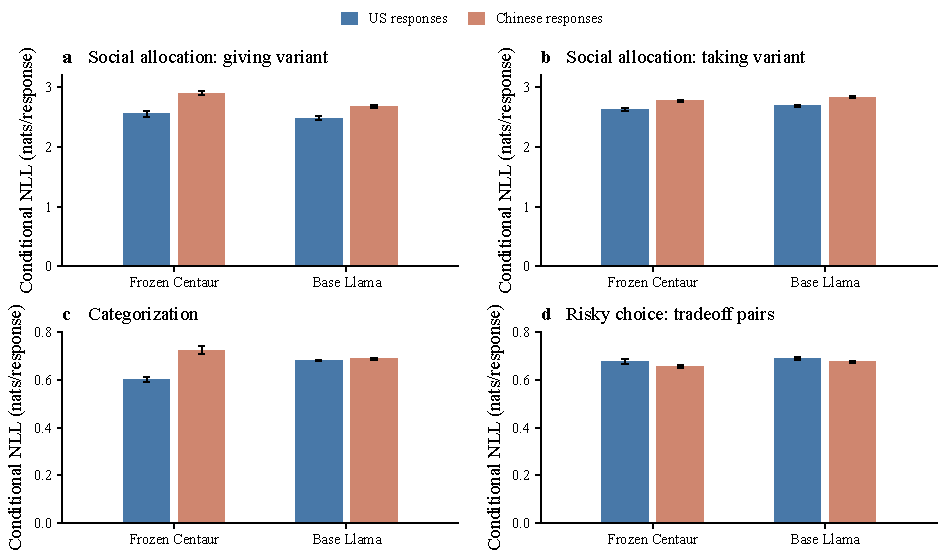
\includegraphics[width=\textwidth]{figures/frozen_sample_fit.pdf}
\caption{Frozen-model conditional NLLs on the samples in Figure~\ref{fig:frozen}; lower is better. Intervals are 95\% participant-bootstrap intervals. Risky-choice scores cover tradeoff pairs. Compare scores within tasks; answer spaces differ across tasks.}
\label{fig:frozen-absolute}
\end{figure}

\begin{table}[htbp]
\centering\small
\setlength{\tabcolsep}{4pt}
\begin{tabular}{llrrrrl}
\toprule
Task & \shortstack{Evaluation\\population} & \shortstack{Frozen\\Centaur} & US & Pooled & China & Matched gain [95\% CI] \\
\midrule
Categorization & US & 0.604 & 0.551 & 0.618 & 0.748 & 0.197 [0.135, 0.256] \\
Categorization & China & 0.721 & 0.877 & 0.719 & 0.700 & 0.177 [0.088, 0.264] \\
Risky choice: tradeoff pairs & US & 0.669 & 0.638 & 0.646 & 0.730 & 0.092 [-0.056, 0.257] \\
Risky choice: tradeoff pairs & China & 0.654 & 0.578 & 0.494 & 0.486 & 0.091 [0.008, 0.168] \\
Risky choice: dominance pairs & US & 0.414 & 0.258 & 0.242 & 0.254 & -0.003 [-0.027, 0.025] \\
Risky choice: dominance pairs & China & 0.380 & 0.169 & 0.149 & 0.155 & 0.014 [-0.013, 0.030] \\
\bottomrule
\end{tabular}
\caption{Mean conditional NLL across three seeds on the same held-out responses. US, Pooled, and China denote fine-tuning populations. Matched gain is opposite-population minus matching-population adapter NLL. Intervals resample participants with fits, seeds, and items fixed.}
\label{tab:extension-scores}
\end{table}

\paragraph{Taking-variant differences by wave.}
The human US--China difference reversed across waves (Table~\ref{tab:taking-waves}). The adapters fine-tuned on the giving variant made the same predictions in both waves, with a mean difference of +1.00 tokens (seed range 0.93--1.14). The transferred difference therefore agreed in direction with wave 1, but not wave 2 or the combined sample.

\begin{table}[H]
\centering\small
\begin{tabular}{lr}
\toprule
Sample & Human US--China difference [95\% CI] \\
\midrule
Wave 1 & $+0.68\ [0.19,\ 1.16]$ \\
Wave 2 & $-1.88\ [-2.28,\ -1.46]$ \\
Combined & $-0.86\ [-1.17,\ -0.54]$ \\
\bottomrule
\end{tabular}
\caption{Differences in mean tokens taken, using 529 participants per country in wave 1 and 800 in wave 2. Intervals resample participants within country and wave.}
\label{tab:taking-waves}
\end{table}

\begin{figure}[H]
\centering
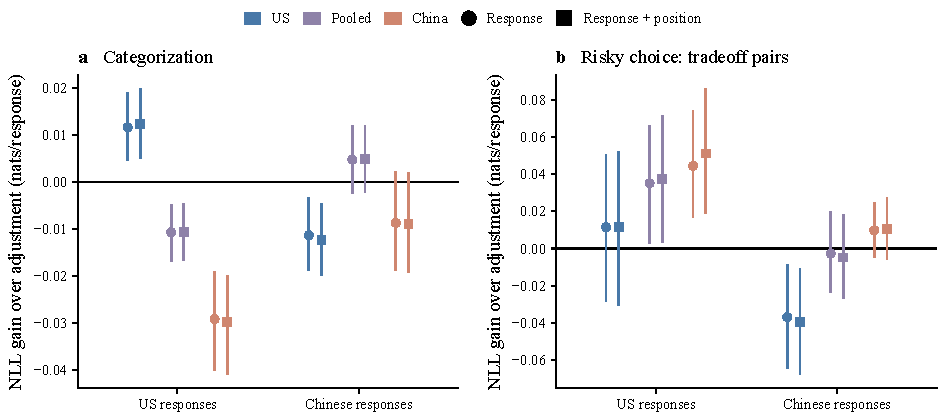
\includegraphics[width=\textwidth]{figures/answer_position_control.pdf}
\caption{NLL gains over response adjustment (circles) or response adjustment with an answer-position parameter (squares). Gains are adjustment NLL minus fine-tuned-model NLL; positive values favor fine-tuning. Each control uses its adapter's training data. Intervals are paired 95\% participant-bootstrap intervals with fits, seeds, and items fixed. Risky-choice results cover tradeoff pairs.}
\label{fig:position-control}
\end{figure}
